%!TEX root = ../../entwurfsprojekt2_entwurfsdokument.tex

\section{Innere Struktur der Komponenten}
\label{sec:struktur}


\subsection{Struktur des Roboterteilsystems (Komponente \texttt{LogisticsRobot})}

\begin{figure}[h]
	\centering
	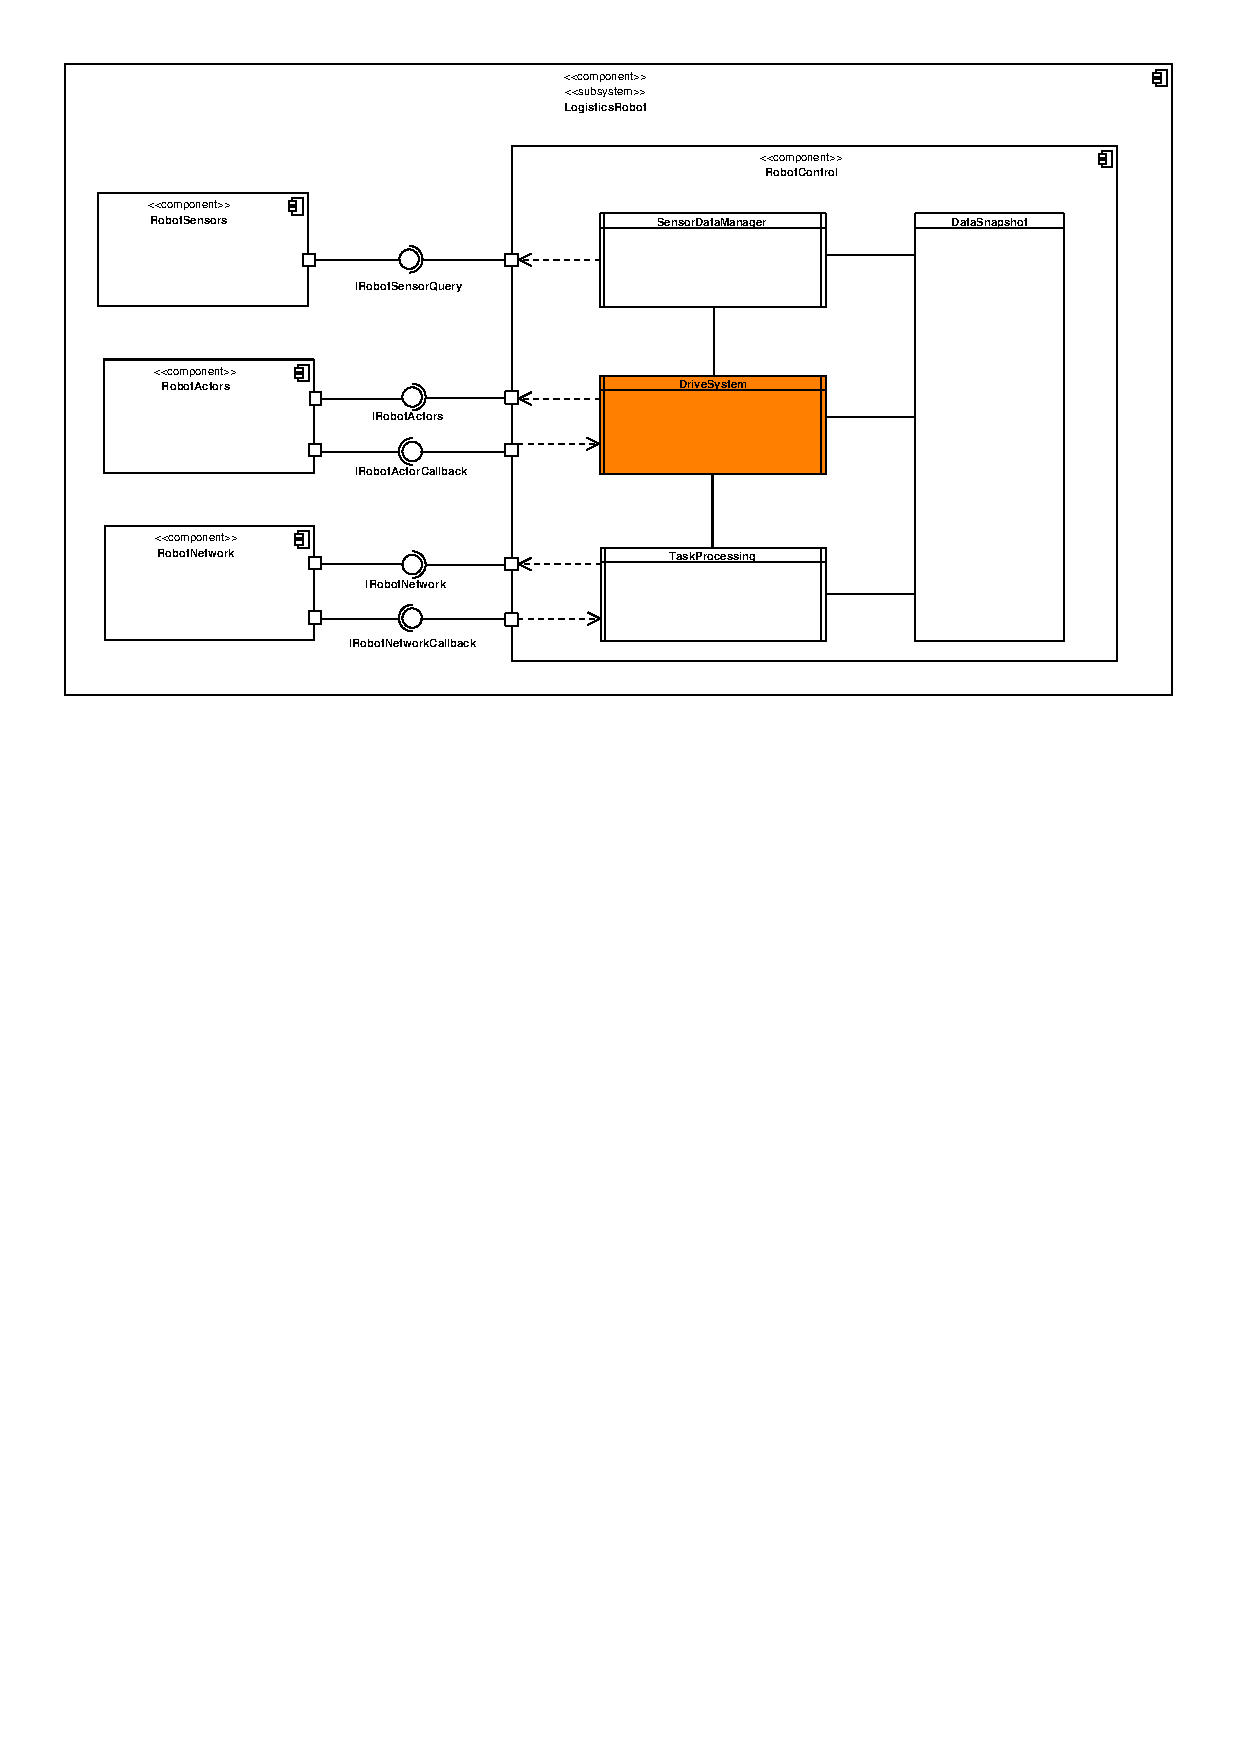
\includegraphics[width=\textwidth]{robot_component_internals}
	\caption{Architektur des Roboterteilsystems.}
	\label{fig:robot_component}
\end{figure}



Auf allen Robotern läuft die gleiche Software (beschrieben durch die gegebene Komponente \texttt{LogisticsRobot}), die sich aus vier Unterkomponenten zusammensetzt (siehe \autoref{fig:robot_component}).

Die Unterkomponente \texttt{RobotControl} ist die zentrale Unterkomponente, die den Roboter steuert. 
Sie enthält die aktive Klasse \texttt{DriveSystem}, welche Zugriff auf die Aktuatoren hat und dadurch das Fahrverhalten eines Roboters bestimmt.
Außerdem beinhaltet die Unterkomponente \texttt{RobotControl} die Klasse \texttt{SensorDataManager} für das Abrufen von Sensordaten, die Klasse \texttt{DataSnapshot} für Speicherung der Sensordaten und die aktive Klasse \texttt{TaskProcessing} für das Empfangen von Aufträgen.


Zur eigentlichen Bewegung stehen physische Aktuatoren zur Verfügung, die von der Unterkomponente \texttt{RobotActors} kontrolliert werden.
Neben Aktuatoren sind auch Sensoren verfügbar. 
Die Messwerte dieser Sensoren stellt die Unterkomponente \texttt{RobotSensors} zur Verfügung.
Die Unterkomponente \texttt{RobotNetwork} wickelt die Kommunikation eines Roboters mit den anderen Teilsystemen ab.